\documentclass[12pt]{article}
\usepackage{worksheet}
\usepackage{graphicx}
\title{Chickens and cages (linear programming problem)}

\begin{document}

\Large

%%%%%%%%%%%%%%%%%%%%%%%%%%%%%%%%%%%%%%%%%%%%%%%%%%%%%%%%%%%%%%%%
\section*{Chickens and cages.}

\subsection*{The Problem.}

You want to buy $x$ chickens and $y$ cages.  But:
\begin{itemize}
\item You need to buy more cages than chickens.
\item You only have \$12; chickens cost \$2 and cages cost \$1.
\end{itemize}
You want to have as many chickens as possible.  How many chickens and
cages should you buy?

\subsection*{The Solution.}

The solution has something to do with the following graph:
\begin{center}
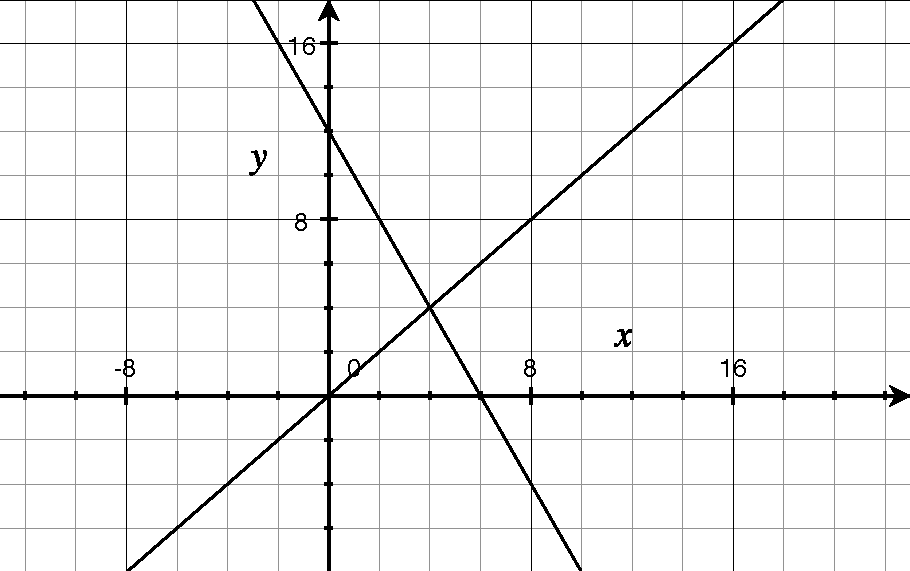
\includegraphics{chicken-inequality-graph.pdf}
\end{center}

Here's a hint:
\begin{itemize}
\item Shade in the region where there are more cages than chickens.
\item Shade in the region where you can afford the combination of chickens and cages.
\end{itemize}

\end{document}
